\documentclass[../../main.tex]{subfiles}

Der Fragenkatalog besteht aus folgenden Fragen:
\begin{enumerate}
    \item Was ist dein Lieblings-Videospliel?
    \item Lieber Single- oder Multiplayer?
    \item Was ist dein Lieblingsgenre?
    \item Was ist deine Lieblingskonsole?
    \item Was ist dein Lieblings-Free-To-Play Spiel?
    \item Eigene Konsole mitnehmen / zur Verfügung gestellte verwenden?
    \item Welches Spiel hast du in Quarantäne am meißten gespielt?
    \item Hast du in Quarantäne mehr Single- oder Multiplayerspiele gespielt?
    \item Wie wichtig sind dir Videospiele?
\end{enumerate}

\begin{tikzpicture}
    \begin{axis}[
        title={Was ist dein lieblings-Videospiel},
        symbolic x coords={
            Among Us,
            Fortnite,
            COD BO4,
            Detroit,
            GTA V,
            LOL,
            Minecraft
        },
        ybar,
        ylabel={Antwortrate [\%]},
        width=\textwidth,
        height=0.4\textheight,
        ymin=0,
        xtick=data,
        x tick label style={rotate=45,anchor=east},
    ]
        \addplot+[ybar] plot coordinates {
            (Among Us,10)
            (Fortnite,16)
            (COD BO4,5)
            (Detroit,5)
            (GTA V,5)
            (LOL,5)
            (Minecraft,15)
        };
    \end{axis}
\end{tikzpicture}

\begin{tikzpicture}
    \begin{axis}[
        title={Lieber Single- oder Multiplayer?},
        symbolic x coords={
            Singleplayer,
            Multiplayer
        },
        ybar,
        ylabel={Antwortrate [\%]},
        width=\textwidth,
        height=0.4\textheight,
        ymin=0,
        xtick=data,
        x tick label style={rotate=45,anchor=east},
    ]
        \addplot+[ybar] plot coordinates {
            (Singleplayer,26)
            (Multiplayer,7)
        };
    \end{axis}
\end{tikzpicture}

\begin{tikzpicture}
    \begin{axis}[
        title={Lieblingsgenre},
        symbolic x coords={
            Action,
            Adventure,
            Role-Playing,
            Simulation,
            Strategie,
            Sport,
            Sandbox,
            Party
        },
        ybar,
        ylabel={Antwortrate [\%]},
        width=\textwidth,
        height=0.4\textheight,
        ymin=0,
        xtick=data,
        x tick label style={rotate=45,anchor=east},
    ]
        \addplot+[ybar] plot coordinates {
            (Action,42)
            (Adventure,11)
            (Role-Playing,5)
            (Simulation,11)
            (Strategie,11)
            (Sport,11)
            (Sandbox,11)
            (Party,0)
        };
    \end{axis}
\end{tikzpicture}

\begin{tikzpicture}
    \begin{axis}[
        title={Lieblingskonsole},
        symbolic x coords={
            PC,
            Playstation,
            Xbox,
            Switch,
            Smartphone
        },
        ybar,
        ylabel={Antwortrate [\%]},
        width=\textwidth,
        height=0.4\textheight,
        ymin=0,
        xtick=data,
        x tick label style={rotate=45,anchor=east},
    ]
        \addplot+[ybar] plot coordinates {
            (PC,32)
            (Playstation,32)
            (Xbox,5)
            (Switch,5)
            (Smartphone,26)
        };
    \end{axis}
\end{tikzpicture}

\begin{tikzpicture}
    \begin{axis}[
        title={Warum diese Konsole?},
        symbolic x coords={
            Tragbar,
            Spielauswahl,
            Vielseitigkeit
        },
        ybar,
        ylabel={Antwortrate [\%]},
        width=\textwidth,
        height=0.4\textheight,
        ymin=0,
        xtick=data,
        x tick label style={rotate=45,anchor=east},
    ]
        \addplot+[ybar] plot coordinates {
            (Tragbar,10)
            (Spielauswahl,10)
            (Vielseitigkeit,15)
        };
    \end{axis}
\end{tikzpicture}

\begin{tikzpicture}
    \begin{axis}[
        title={Lieblings Free-To-Play-Spiel},
        symbolic x coords={
            Among Us,
            COD Mobile,
            Fortnite,
            Paladins,
            Roblox,
            Rocket League,
            The Wolf
        },
        ybar,
        ylabel={Antwortrate [\%]},
        width=\textwidth,
        height=0.4\textheight,
        ymin=0,
        xtick=data,
        x tick label style={rotate=45,anchor=east},
    ]
        \addplot+[ybar] plot coordinates {
            (Among Us,15)
            (COD Mobile,5)
            (Fortnite,21)
            (Paladins,5)
            (Roblox,5)
            (Rocket League,5)
            (The Wolf,5)
        };
    \end{axis}
\end{tikzpicture}

\begin{tikzpicture}
    \begin{axis}[
        title={Lieber eigene Konsole mitnehmen (A) oder zur Verfügung gestellte (B) verwenden?},
        symbolic x coords={
            A,
            B
        },
        ybar,
        ylabel={Antwortrate [\%]},
        width=\textwidth,
        height=0.4\textheight,
        ymin=0,
        xtick=data,
        x tick label style={rotate=45,anchor=east},
    ]
        \addplot+[ybar] plot coordinates {
            (A,74)
            (B,26)
        };
    \end{axis}
\end{tikzpicture}

\begin{tikzpicture}
    \begin{axis}[
        title={Welches Spiel hast du in Quarantäne am meißten gespielt?},
        symbolic x coords={
            COD Mobile,
            Fortnite,
            GTA V,
            LOL,
            Minecraft,
            Roblox,
            Rocket League
        },
        ybar,
        ylabel={Antwortrate [\%]},
        width=\textwidth,
        height=0.4\textheight,
        ymin=0,
        xtick=data,
        x tick label style={rotate=45,anchor=east},
    ]
        \addplot+[ybar] plot coordinates {
            (COD Mobile,5)
            (Fortnite,21)
            (GTA V,5)
            (LOL,5)
            (Minecraft,10)
            (Roblox,5)
            (Rocket League,5)
        };
    \end{axis}
\end{tikzpicture}

\begin{tikzpicture}
    \begin{axis}[
        title={Hast du in Quarantäne mehr Single- oder Multiplayerspiele gespielt?},
        symbolic x coords={
            Singleplayer,
            Multiplayer
        },
        ybar,
        ylabel={Antwortrate [\%]},
        width=\textwidth,
        height=0.4\textheight,
        ymin=0,
        xtick=data,
        x tick label style={rotate=45,anchor=east},
    ]
        \addplot+[ybar] plot coordinates {
            (Singleplayer,42)
            (Multiplayer,58)
        };
    \end{axis}
\end{tikzpicture}

\begin{tikzpicture}
    \begin{axis}[
        title={Mir sind Videospiele sehr wichtig und ich verbringe meine Freizeit damit.},
        symbolic x coords={
            Trifft sehr zu,
            Trifft eher zu,
            Trifft eher nicht zu,
            Trifft nicht zu
        },
        ybar,
        ylabel={Antwortrate [\%]},
        width=\textwidth,
        height=0.4\textheight,
        ymin=0,
        xtick=data,
        x tick label style={rotate=45,anchor=east},
    ]
        \addplot+[ybar] plot coordinates {
            (Trifft sehr zu,16)
            (Trifft eher zu,37)
            (Trifft eher nicht zu,37)
            (Trifft nicht zu,11)
        };
    \end{axis}
\end{tikzpicture}